\section{Explaining, Stress-Testing and Verifying the Method}\label{sec:round3}

This section adds a third round of analysis: tools that explain \emph{what} compliance costs
and \emph{why} CA-HRP is stable, a stress test of the evidence against the objection that the
constraint sets were hand-picked, stricter statistics, and an independent verification of the
implementation.

\subsection{What does compliance cost, and which rule is responsible?}
Using Proposition~\ref{prop:kkt} and the Shapley split we decompose, on every one of the
1{,}363 CA-HRP rebalances, the tracking error that compliance forces away from HRP
(Table~\ref{tab:compliance}, Figure~\ref{fig:compliance}). Two checks hold on every date:
re-solving the attribution problem from scratch reproduces the stored backtest weights to
within $2.4\times10^{-10}$, and the turnover remainder in \eqref{eq:kkt} is below
$10^{-8}$ whenever the turnover cap is slack, as the identity requires.

The price of compliance differs sharply across mandates. In the multi-asset universe CA-HRP
must sit 5.0\% (ex-ante tracking error, p.a.) away from HRP on average, and 14.6\% at the peak
in 2009, when HRP wanted almost the entire portfolio in short-term Treasuries. In the stock
universes compliance is nearly free (0.1\% on average) and costs nothing at all on 59\%
(NIFTY) and 41\% (US) of rebalance dates. Wherever compliance is expensive, \emph{group}
limits are responsible for most of it: 67\% of the cost for multi-asset ETFs, 73\% for US
sectors, 77\% for countries and 82\% for Indian ETFs. Only in the NIFTY universe, where sector
caps are loose relative to the index, do single-stock caps dominate (97\%). The turnover cap
binds on at most 12\% of dates; its 20\% Shapley share in the multi-asset universe reflects
that, on its own, a turnover budget would also stop the portfolio from moving towards a target
that the other limits have already pushed far away, which the Shapley value credits to it.
This attribution is, to our knowledge, new for hierarchical allocation and gives a portfolio
manager a direct answer to ``which rule of my mandate is costing me the most HRP-ness?''.

\begin{table}[!htbp]\centering\small
\caption{Price of compliance for CA-HRP: ex-ante tracking error to HRP (\% p.a.) needed to satisfy the mandate, share of rebalances where compliance is free, share where the turnover cap binds, and the Shapley split of the cost across constraint families.}\label{tab:compliance}
\setlength{\tabcolsep}{4pt}\begin{tabular}{l rrrr rrr}\toprule
 & \multicolumn{2}{c}{TE to HRP} & Free & Turnover & \multicolumn{3}{c}{Shapley share}\\
\cmidrule(lr){2-3}\cmidrule(lr){6-8}
Universe & mean & max & dates & binds & asset caps & groups & turnover\\\midrule
ETFs & 5.0 & 14.6 & 0\% & 1\% & 14\% & 67\% & 20\%\\
NIFTY & 0.1 & 0.5 & 59\% & 7\% & 97\% & 1\% & 2\%\\
US & 0.1 & 0.9 & 41\% & 6\% & 46\% & 51\% & 3\%\\
India ETFs & 2.8 & 6.8 & 3\% & 3\% & 13\% & 82\% & 5\%\\
US sectors & 1.0 & 3.8 & 10\% & 12\% & 24\% & 73\% & 3\%\\
Countries & 0.7 & 2.2 & 2\% & 11\% & 22\% & 77\% & 1\%\\
\bottomrule\end{tabular}\end{table}

\begin{figure}[!htbp]
\centering
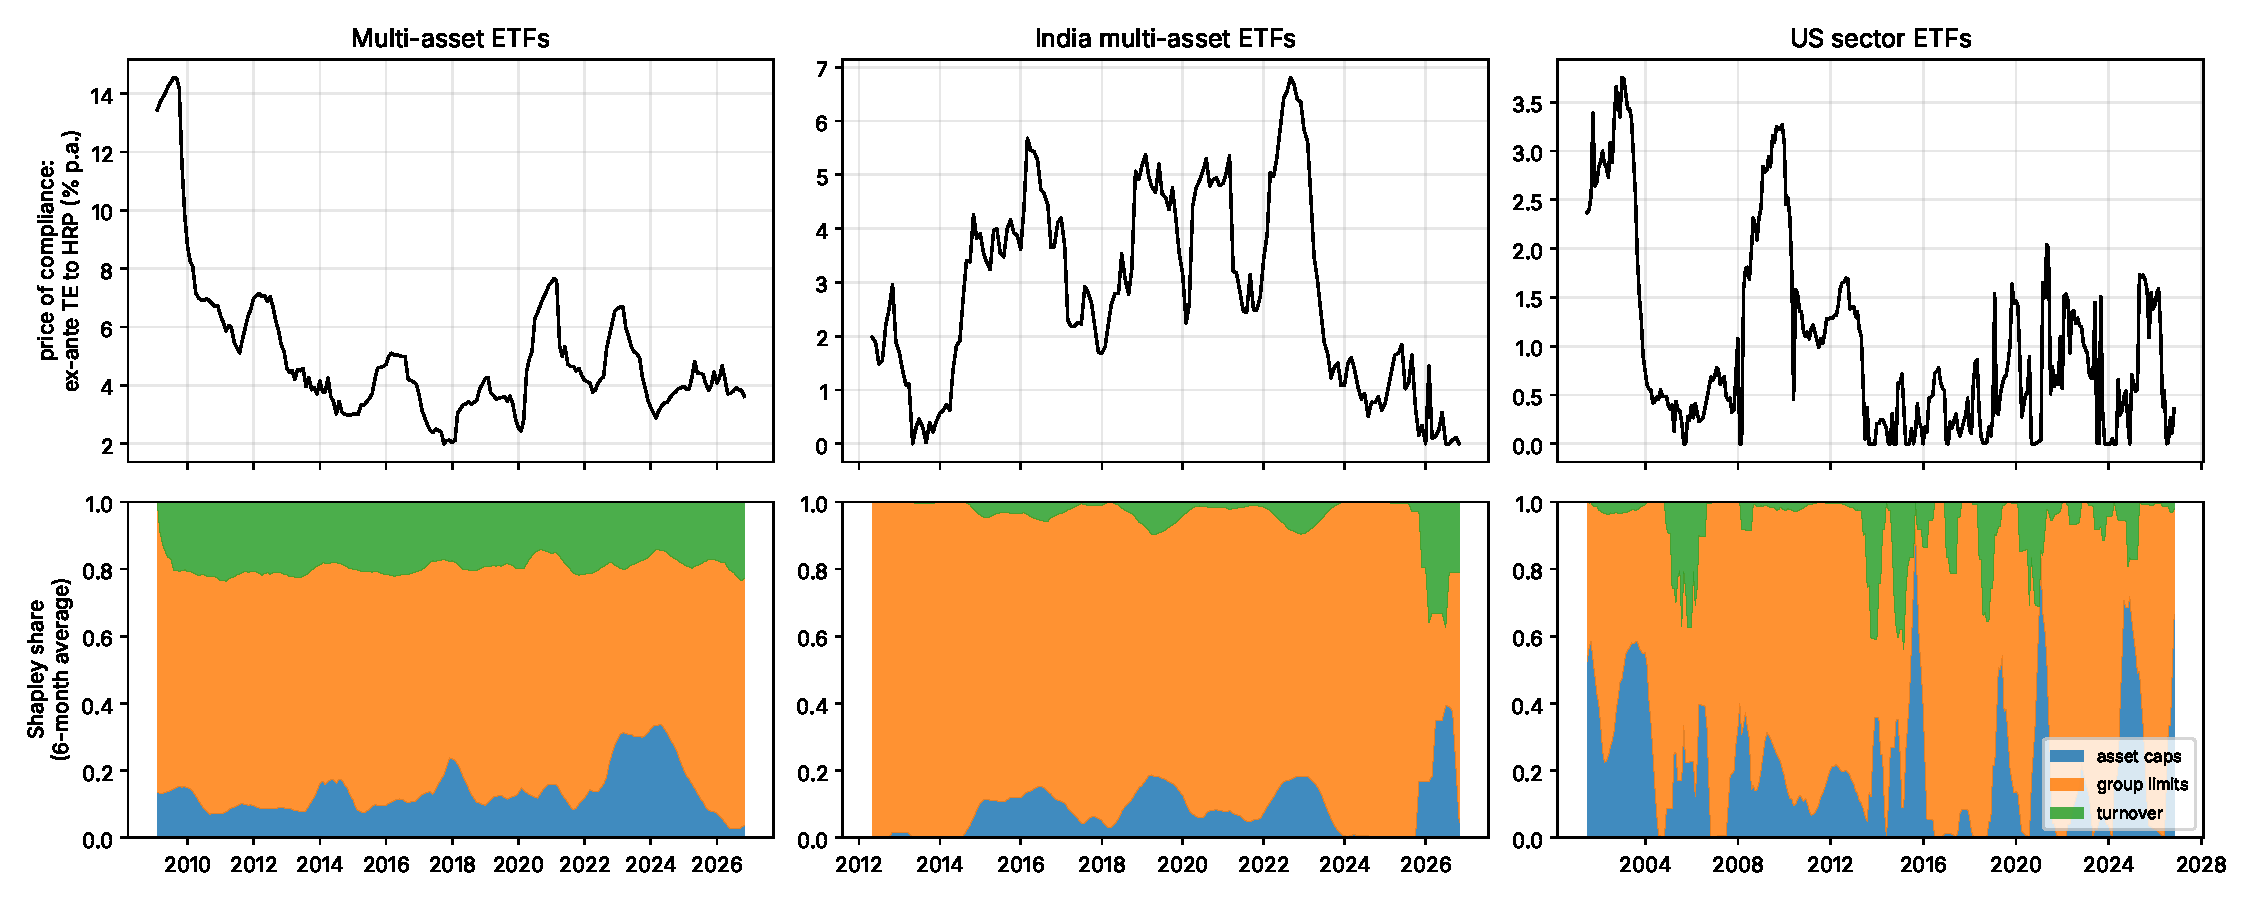
\includegraphics[width=\linewidth]{../results/figures/compliance_cost.pdf}
\caption{Top: price of compliance (ex-ante tracking error of CA-HRP to HRP). Bottom: Shapley
share of each constraint family (6-month moving average).}
\label{fig:compliance}
\end{figure}

\subsection{Noise damping: CA-HRP shrinks estimation noise, clipping amplifies it}
To test Proposition~\ref{prop:nonexp} empirically we bootstrap the estimation window 40 times
at 10 dates per universe, compute HRP on each resample, and push each target through the
CA-HRP projection and through HRP-Clip. For all $6\times10\times780$ pairs of resamples we
compare the distance between the two portfolios with the distance between the two targets
(Table~\ref{tab:noise}). The CA-HRP projection never increased the distance beyond solver
tolerance (largest ratio $1+10^{-6}$), as the proposition guarantees, and on average it
shrank it, to 0.48 of its original size for multi-asset ETFs and to 0.74--0.97 elsewhere.
Clipping behaves very differently. In the multi-asset universe it amplified noise on average
(ratio 2.08) and by a factor of 10.5 for the worst pair, and it pushed half of all pairs
further apart; in the Indian ETF and sector universes it amplified 43\% and 25\% of pairs.
This is the mechanism behind HRP-Clip's high turnover in Table~\ref{tab:main}: small changes
in the estimate produce large changes in the clipped portfolio.

\begin{table}[!htbp]\centering\small
\caption{Noise damping. Ratio of the dispersion of bootstrapped portfolios to the dispersion of the bootstrapped HRP targets (1 = noise passed through unchanged, $<$1 = damped, $>$1 = amplified), averaged over 10 dates $\times$ 780 bootstrap pairs, and the worst pair. Measured in the risk metric $\bar\Sigma$; ``share amplified'' is the fraction of pairs that clipping pushes further apart in the Euclidean norm.}\label{tab:noise}
\setlength{\tabcolsep}{4pt}\begin{tabular}{l rr rr r}\toprule
 & \multicolumn{2}{c}{CA-HRP projection} & \multicolumn{2}{c}{HRP-Clip} & Share\\
\cmidrule(lr){2-3}\cmidrule(lr){4-5}
Universe & mean & worst & mean & worst & amplified\\\midrule
ETFs & 0.48 & 0.99 & 2.08 & 10.49 & 50\%\\
NIFTY & 0.97 & 1.00 & 0.96 & 1.06 & 3\%\\
US & 0.97 & 1.00 & 0.95 & 1.17 & 4\%\\
India ETFs & 0.74 & 1.00 & 0.90 & 1.99 & 43\%\\
US sectors & 0.85 & 1.00 & 0.84 & 1.75 & 25\%\\
Countries & 0.82 & 1.00 & 0.83 & 1.63 & 14\%\\
\bottomrule\end{tabular}\end{table}

\subsection{Random mandates and a placebo test}
The constraint sets in Sections~\ref{sec:results}--\ref{sec:extended} were fixed in advance,
but they are still only nine mandates. To remove any suspicion that they favour CA-HRP, we
drew 160 random mandates, 40 in each of four universes (multi-asset ETFs, NIFTY, US large
caps and countries). Each draw picks a random subset of between half and all of the assets, a
random start date in the first third of the sample, a per-asset cap between $1.5/n$ and $4/n$,
a group cap between $1.2/G$ and $2.5/G$, and a 30\% turnover budget; infeasible draws are
rejected by a linear feasibility check. As a placebo, every second draw replaces the true
sector, asset-class or region labels by random labels into three to six groups, which breaks
the link between groups and correlation structure. The design and random seeds were fixed
before the study was run.

Table~\ref{tab:random} and Figure~\ref{fig:random} summarise the results. CA-HRP and the
other optimisation-based methods satisfied every constraint in every mandate, while HRP-Clip
breached them at 4\% of rebalances. CA-HRP had volatility no higher than HRP-Proj in 85\% of
the mandates. On Sharpe ratio, however, the picture is balanced: CA-HRP beat HRP-Proj in
55\% of mandates (mean difference $+0.014$, median $+0.002$), HRP-Clip in 56\% and
constrained minimum variance in 46\%. The advantage is concentrated in the multi-asset
universe, where CA-HRP beat HRP-Proj in 90\% of mandates with true groups, and it reverses
for country funds, where it won only 25--30\% of the time. Scrambling the group labels halves
the multi-asset advantage ($+0.076$ to $+0.035$), consistent with the mechanism of
Proposition~\ref{prop:te}(d): when groups follow the correlation structure, choosing
replacement assets by covariance matters more. In the US universe the placebo did not weaken
the effect, so this evidence is suggestive rather than conclusive. The gain is largest when HRP
breaches the mandate at more than 75\% of rebalances ($+0.021$, 60\% win rate), but it is not
monotone in how often the mandate binds. Overall the random mandates support the paper's
central, narrower claim: CA-HRP is a reliable and lower-risk way to make HRP compliant, with
a return advantage that is specific to strongly binding, correlation-aligned group
constraints.

\begin{table}[!htbp]\centering\small
\caption{Random mandates (40 per universe, half with scrambled group labels). Share of mandates in which CA-HRP has a higher Sharpe ratio than each competitor, mean Sharpe difference with HRP-Proj, and share in which CA-HRP's volatility is not higher than HRP-Proj's.}\label{tab:random}
\setlength{\tabcolsep}{3.5pt}\begin{tabular}{ll r rrr r r}\toprule
Universe & Groups & $n$ & \multicolumn{3}{c}{CA-HRP wins vs} & $\Delta$SR & Vol $\le$\\
\cmidrule(lr){4-6}
 & & & Proj & Clip & MinVar-C & vs Proj & Proj\\\midrule
Countries & true & 20 & 30\% & 25\% & 30\% & -0.002 & 90\%\\
Countries & scrambled & 20 & 25\% & 30\% & 25\% & -0.005 & 90\%\\
ETFs & true & 20 & 90\% & 95\% & 10\% & +0.076 & 100\%\\
ETFs & scrambled & 20 & 75\% & 95\% & 30\% & +0.035 & 100\%\\
NIFTY & true & 20 & 45\% & 40\% & 70\% & +0.001 & 70\%\\
NIFTY & scrambled & 20 & 45\% & 40\% & 55\% & -0.002 & 40\%\\
US & true & 20 & 60\% & 55\% & 65\% & +0.002 & 95\%\\
US & scrambled & 20 & 70\% & 70\% & 85\% & +0.009 & 95\%\\
All & all & 160 & 55\% & 56\% & 46\% & +0.014 & 85\%\\
\midrule
\multicolumn{8}{l}{\emph{By how often HRP breaches the mandate:}}\\
\multicolumn{2}{l}{HRP breach share (-0.01, 0.25]} & 21 & 48\% & & & +0.004 & \\
\multicolumn{2}{l}{HRP breach share (0.25, 0.5]} & 17 & 59\% & & & +0.007 & \\
\multicolumn{2}{l}{HRP breach share (0.5, 0.75]} & 21 & 33\% & & & -0.004 & \\
\multicolumn{2}{l}{HRP breach share (0.75, 1.0]} & 101 & 60\% & & & +0.021 & \\
\bottomrule\end{tabular}\end{table}

\begin{figure}[!htbp]
\centering
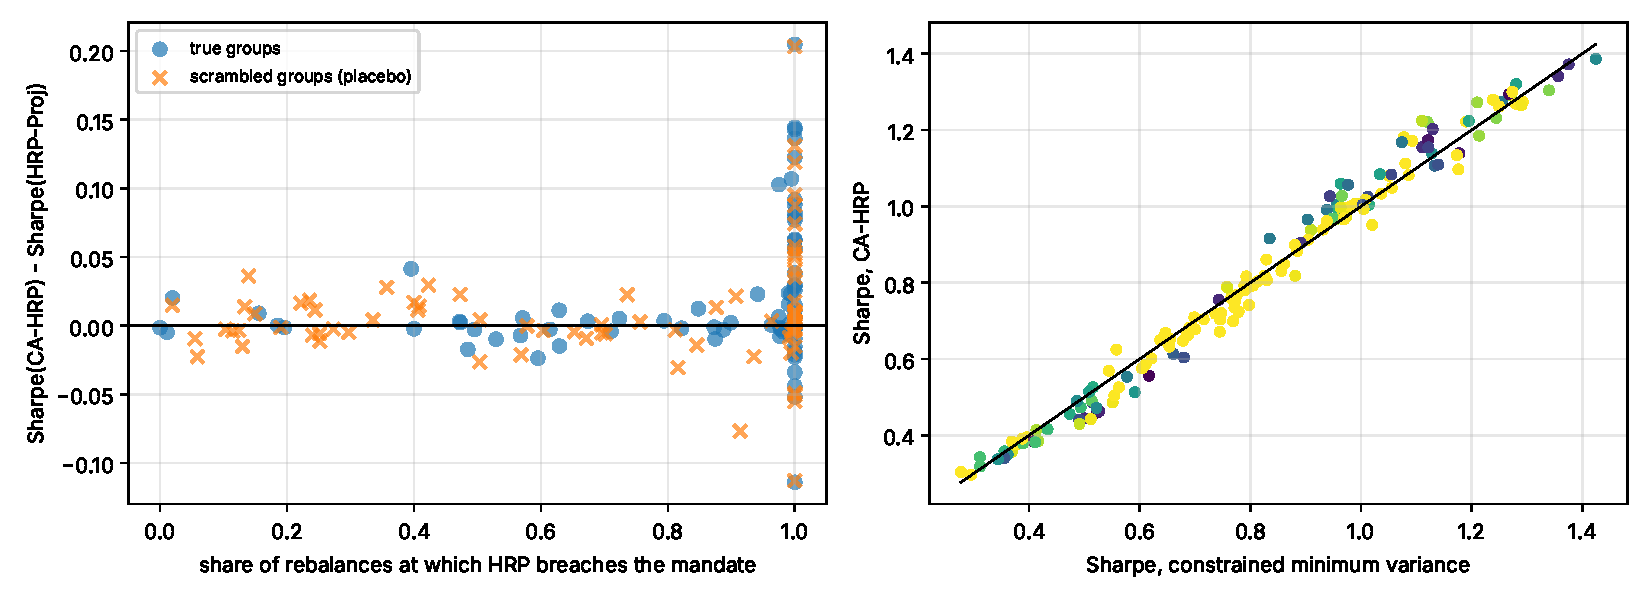
\includegraphics[width=\linewidth]{../results/figures/random_mandates.pdf}
\caption{Random mandates. Left: Sharpe-ratio gain of CA-HRP over HRP-Proj against how often
HRP breaches the mandate (circles: true groups; crosses: scrambled-group placebo). Right:
CA-HRP against constrained minimum variance (colour: HRP breach share).}
\label{fig:random}
\end{figure}


\subsection{Forward-looking risk from option-implied volatility}\label{sec:iv}
All risk inputs so far are backward-looking. Option prices, by contrast, embed the market's
forward-looking view of volatility, which often moves before realised volatility does. We
therefore test a variant, CA-HRP-IV, that keeps the historical (Ledoit--Wolf) correlations
but rescales each asset's volatility by the implied-to-realised ratio of the volatility index
of its asset class:
\begin{equation}\label{eq:iv}
\sigma_i^{\mathrm{IV}}(d)=\sigma_i^{\mathrm{hist}}(d)\,\frac{\mathrm{IV}_{k(i)}(d^-)}{\mathrm{RV}_{k(i)}(d^-)},
\end{equation}
where $\mathrm{IV}_k$ is the index level on the last trading day strictly before the
rebalance date $d$ and $\mathrm{RV}_k$ the realised volatility of its underlying over the 252
preceding days. We use VIX (US and international equity and real estate), VXN (Nasdaq-100),
GVZ (gold and silver), OVX (oil and broad commodities), MOVE (Treasuries and investment-grade
credit, with realised volatility measured on daily 10-year yield changes in basis points) and
India VIX (Indian equity). Assets without a suitable index (high-yield and emerging-market
bonds) receive the median ratio of the available indices, so that the variance risk premium
does not make them look artificially safe. The resulting covariance replaces the historical
one in both the HRP allocation and the projection metric. The one-day lag avoids look-ahead
across time zones, and the mapping was fixed before any backtest. To attribute any effect to
the \emph{information} rather than the method, the same covariance is also given to
constrained minimum variance (MinVar-C-IV).

\begin{proposition}[Scale invariance]\label{prop:scale}
HRP weights and the CA-HRP projection are unchanged when every volatility is multiplied by
the same factor $\kappa>0$.
\end{proposition}
\begin{proof}
Correlations, and therefore the tree, are unchanged. Every cluster variance in
\eqref{eq:alpha} scales by $\kappa^2$, so the split fractions do not change. The projection
metric in \eqref{eq:te} is normalised by its trace, which removes $\kappa^2$.
\end{proof}

Proposition~\ref{prop:scale} implies that option information can only change CA-HRP through
the \emph{relative} implied/realised ratios across asset classes, so a single index such as
VIX applied to a one-asset-class universe would have no effect; this is why we test it on the
two multi-asset universes. Both properties, together with the absence of look-ahead in
\eqref{eq:iv}, are covered by unit tests, and with the ratios set to one the IV code path
reproduces CA-HRP exactly.

The ratios vary widely (Figure~\ref{fig:iv}): at month-ends they peaked at 2.9 for VIX
(February 2020), 3.3 for OVX and 3.1 for India VIX (March 2020), and during 2022 MOVE was on
average 25\% above realised Treasury volatility (monthly range 0.97--1.55). Table~\ref{tab:iv} shows the outcome, which is mixed. Option information did not change
risk-adjusted returns: CA-HRP-IV has a Sharpe ratio of 0.907 against 0.908 for CA-HRP in the
multi-asset universe and 1.280 against 1.276 for Indian ETFs, with intervals centred on zero.
It did improve crash behaviour in the US multi-asset universe, cutting the COVID-crash loss
from 6.9\% to 5.5\% and the 2022 loss from 17.2\% to 16.4\%, but it worsened the COVID loss for
Indian ETFs (7.9\% against 5.3\%). It also roughly doubled turnover (2.10 against 1.25 and 1.91
against 0.98 per year), because implied/realised ratios move from month to month.
Constrained minimum variance benefited somewhat more from the same information (Sharpe 1.355
against 1.321 for Indian ETFs). We conclude that implied volatility is a usable, look-ahead-free
input to CA-HRP whose benefit is limited to some crisis episodes; smoothing the ratios to
contain turnover is a natural extension, which we leave for future work rather than tune on
these data.

\begin{table*}[!htbp]\centering\small
\caption{Forward-looking risk with option-implied volatility (net of 10\,bps). CA-HRP-IV and MinVar-C-IV use historical correlations and volatilities rescaled by implied/realised ratios of VIX, VXN, GVZ, OVX, MOVE and India VIX. Vol, MaxDD and stress returns in \%; $\Delta$SR = Sharpe of CA-HRP-IV minus that method, with 95\% block-bootstrap interval.}\label{tab:iv}
\resizebox{\linewidth}{!}{\begin{tabular}{ll rrrrr rrr c}\toprule
Universe & Method & Sharpe & Test SR & Vol & MaxDD & Turn. & GFC & COVID & 2022 & $\Delta$SR [95\% CI]\\\midrule
\multirow{5}{*}{Multi-asset ETFs} & HRP-Proj & 0.764 & 0.805 & 9.9 & -22.8 & 0.62 & -1.0 & -14.0 & -15.3 & +0.143 [-0.07, +0.34]\\
 & MinVar-C & 0.935 & 0.977 & 7.3 & -17.5 & 1.21 & 0.5 & -7.6 & -16.0 & -0.028 [-0.13, +0.07]\\
 & MinVar-C-IV & 0.932 & 0.959 & 7.3 & -17.1 & 1.96 & 0.1 & -5.7 & -15.2 & -0.025 [-0.08, +0.03]\\
 & CA-HRP & 0.908 & 0.929 & 7.4 & -18.8 & 1.25 & 0.3 & -6.9 & -17.2 & -0.001 [-0.09, +0.08]\\
 & \textbf{CA-HRP-IV} & 0.907 & 0.913 & 7.3 & -18.3 & 2.10 & 0.1 & -5.5 & -16.4 & --\\
\midrule
\multirow{5}{*}{India ETFs} & HRP-Proj & 1.257 & -- & 11.9 & -25.6 & 0.69 & -- & -7.1 & 2.7 & +0.023 [-0.11, +0.15]\\
 & MinVar-C & 1.321 & -- & 10.9 & -24.9 & 0.79 & -- & -4.0 & -1.8 & -0.041 [-0.16, +0.07]\\
 & MinVar-C-IV & 1.355 & -- & 10.9 & -26.2 & 1.74 & -- & -6.4 & -2.1 & -0.076 [-0.17, +0.01]\\
 & CA-HRP & 1.276 & -- & 11.3 & -24.9 & 0.98 & -- & -5.3 & -2.3 & +0.004 [-0.09, +0.09]\\
 & \textbf{CA-HRP-IV} & 1.280 & -- & 11.2 & -26.6 & 1.91 & -- & -7.9 & -2.1 & --\\
\bottomrule
\end{tabular}}\end{table*}

\begin{figure}[!htbp]
\centering
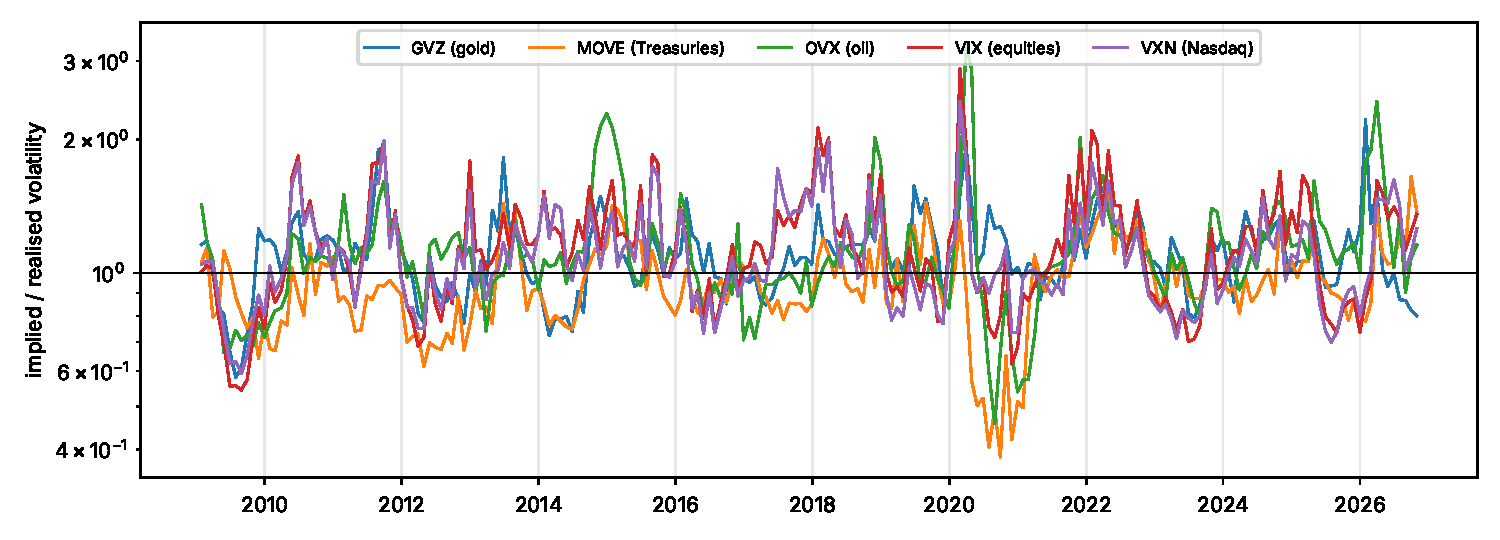
\includegraphics[width=\linewidth]{../results/figures/iv_ratios.pdf}
\caption{Implied-to-realised volatility ratios used by CA-HRP-IV in the multi-asset universe
(log scale; 1 = implied equals realised).}
\label{fig:iv}
\end{figure}

\subsection{Stricter statistics}
\paragraph{Model Confidence Set.} Table~\ref{tab:stats} applies the Model Confidence Set of
\citet{hansen2011} (T$_{\max}$ statistic, 21-day block bootstrap, 1{,}000 draws, 90\%
level) to the six mandate-compliant methods. With negative returns as the loss, no method can
be eliminated in any universe: realised returns cannot distinguish these methods over 15--25
years. With squared returns as the loss, constrained minimum variance is in the set in every
universe, as it should be since it minimises variance by design; CA-HRP and CA-HRP-R are the
only other methods that survive, and only in the multi-asset universe.

\paragraph{Deflated Sharpe ratio.} During the project we evaluated 22 configurations of
CA-HRP (design study, robust design study and ablations). Charging for all of them with the
deflated Sharpe ratio of \citet{bailey2014} (using the cross-method variance of
Sharpe ratios, which is conservative), CA-HRP's Sharpe ratio remains significantly positive
in every universe (DSR between 0.963 for countries and 1.000), despite strongly fat-tailed
returns (daily kurtosis 9--20). Its positive risk-adjusted return is therefore not an
artefact of trying many variants, although, as above, this is not evidence of superiority over
the other compliant methods.

\paragraph{Risk calibration.} Optimised portfolios tend to under-predict their own risk. We
compare each method's predicted volatility at each rebalance with the realised volatility of
the following month. Constrained minimum variance is the most optimistic in the stock
universes (bias statistic 1.29 for NIFTY and 1.12 for US, against 1.21 and 1.05 for CA-HRP),
consistent with the optimiser's curse; in the ETF universes the methods are similar
(1.03--1.15). CA-HRP's risk forecasts are therefore at least as reliable as those of the
optimisers it is compared with, which matters to a risk manager even when realised returns
are indistinguishable.

\begin{table*}[!htbp]\centering\small
\caption{Statistical checks. Left: membership of the 90\% Model Confidence Set (\checkmark) for return (negative return loss) and risk (squared return loss) among the mandate-compliant methods. Middle: CA-HRP's probabilistic Sharpe ratio against zero and its deflated Sharpe ratio after charging for 22 configurations tried. Right: risk calibration bias statistic (standard deviation of monthly returns standardised by predicted risk; 1 = calibrated, $>$1 = risk under-predicted).}\label{tab:stats}
\resizebox{\linewidth}{!}{\begin{tabular}{l cccccc cccccc rr rrr}\toprule
 & \multicolumn{6}{c}{MCS (return)} & \multicolumn{6}{c}{MCS (risk)} & \multicolumn{2}{c}{CA-HRP} & \multicolumn{3}{c}{Bias statistic}\\
\cmidrule(lr){2-7}\cmidrule(lr){8-13}\cmidrule(lr){14-15}\cmidrule(lr){16-18}
Universe & \rotatebox{90}{MinVar-C} & \rotatebox{90}{MVO-C} & \rotatebox{90}{HRP-Proj} & \rotatebox{90}{CA-HRP-B} & \rotatebox{90}{CA-HRP} & \rotatebox{90}{CA-HRP-R} & \rotatebox{90}{MinVar-C} & \rotatebox{90}{MVO-C} & \rotatebox{90}{HRP-Proj} & \rotatebox{90}{CA-HRP-B} & \rotatebox{90}{CA-HRP} & \rotatebox{90}{CA-HRP-R} & PSR & DSR & MinVar-C & HRP-Proj & CA-HRP\\\midrule
ETFs & \checkmark & \checkmark & \checkmark & \checkmark & \checkmark & \checkmark & \checkmark &  &  &  & \checkmark & \checkmark & 1.000 & 0.999 & 1.08 & 1.05 & 1.08\\
NIFTY & \checkmark & \checkmark & \checkmark & \checkmark & \checkmark & \checkmark & \checkmark &  &  &  &  &  & 1.000 & 1.000 & 1.29 & 1.21 & 1.20\\
US & \checkmark & \checkmark & \checkmark & \checkmark & \checkmark & \checkmark & \checkmark &  &  &  &  &  & 1.000 & 1.000 & 1.12 & 1.05 & 1.05\\
India ETFs & \checkmark & \checkmark & \checkmark & \checkmark & \checkmark & \checkmark & \checkmark &  &  &  &  &  & 1.000 & 1.000 & 1.13 & 1.14 & 1.13\\
US sectors & \checkmark & \checkmark & \checkmark & \checkmark & \checkmark & \checkmark & \checkmark &  &  &  &  &  & 0.999 & 0.998 & 1.00 & 0.97 & 0.98\\
Countries & \checkmark & \checkmark & \checkmark & \checkmark & \checkmark & \checkmark & \checkmark &  &  &  &  &  & 0.975 & 0.963 & 1.02 & 0.99 & 1.00\\
\bottomrule\end{tabular}}\end{table*}

\subsection{Verification}
Table~\ref{tab:verify} lists eleven automated checks run against the stored results. Our HRP
implementation reproduces the independent PyPortfolioOpt implementation \citep{martin2021} to $10^{-16}$ on
36 windows. No look-ahead: replacing every return after a given date by random noise leaves
all earlier weights and returns bit-for-bit unchanged. Re-running backtests reproduces the
stored results exactly; transaction costs, Sharpe ratios, growth rates and drawdowns
recomputed by independent code agree to $10^{-15}$; the tables in the paper equal a fresh
recomputation; three different solvers agree on the projection to $6\times10^{-5}$; and an
audit of every stored portfolio of every compliant method finds no constraint breached by
more than $2\times10^{-8}$. One check failed its strict threshold: our constrained
minimum-variance solutions have up to $1.8\times10^{-4}$ relative excess variance over
PyPortfolioOpt's, because daily variances are tiny relative to default solver tolerances.
Re-solving with a rescaled objective changes that competitor's Sharpe ratio by at most
$3\times10^{-4}$, so no conclusion depends on it; we keep the original numbers so that the
repository reproduces every table exactly. A SHA-256 manifest of all data files is included
in the repository.

\begin{table*}[!htbp]\centering\small
\caption{Verification suite (\texttt{scripts/verify.py}). Every check is run on the stored results; the one strict failure is reported together with its economic impact.}\label{tab:verify}
\footnotesize\begin{tabular}{p{3.4cm}p{7.4cm}rrc}\toprule
Check & What is measured & Value & Threshold & Result\\\midrule
Data manifest written & SHA-256 of every raw data file & 0 & 0 & pass\\
No look-ahead & weights up to a date unchanged when all later returns are replaced by noise & 0 & 0 & pass\\
Deterministic re-run & max diff vs stored results (2 universes $\times$ 3 methods) & 0 & 1e-09 & pass\\
Cost accounting & $|$(gross - net) - turnover $\times$ cost$|$ summed per backtest, max & 5.6e-16 & 1e-10 & pass\\
Independent metric recomputation & max gap in Sharpe / CAGR / MaxDD, all backtests & 4.4e-16 & 1e-09 & pass\\
Paper tables match raw results & max gap Sharpe/Vol between table CSV and recomputation & 2.2e-16 & 1e-12 & pass\\
Raw constraint audit & largest breach of any constraint, 6 compliant methods $\times$ 6 universes, no tolerance & 2.2e-08 & 1e-06 & pass\\
Three solvers agree & max weight gap CLARABEL vs OSQP/SCS, 30 projections & 5.7e-05 & 1e-04 & pass\\
HRP matches PyPortfolioOpt & max $|$w\_ours - w\_ref$|$ over 36 windows, 6 universes & 1.1e-16 & 1e-08 & pass\\
Min-variance matches PyPortfolioOpt & max relative excess variance of our solution over the reference, 36 windows & 1.8e-04 & 1e-04 & \textbf{fail}\\
Min-variance precision: economic impact & max change in MinVar-C Sharpe when re-solved with a rescaled objective, 6 universes & 2.7e-04 & 1e-03 & pass\\
\bottomrule\end{tabular}\end{table*}
